\documentclass[12pt,a4paper]{exam}

\usepackage[utf8]{inputenc}
\usepackage[T1]{fontenc}
\usepackage[french]{babel}
\usepackage{amsmath,amssymb}
\usepackage{pgfplots}
\pgfplotsset{compat=1.18}
\usepackage{tikz}
\usepackage{multicol}
\usetikzlibrary{arrows.meta}
\usepackage{geometry}
\usepackage{graphicx}
\usepackage{xcolor}
\geometry{margin=2cm}

\setlength{\parindent}{0pt}

\begin{document}

\begin{center}
\Large \textbf{-Interrogation-\\Écriture fractionnaire (401)}
\vspace{0.5cm}
\\\large \underline{\textbf{JUSTIFIER VOS RÉPONSES SUR VOTRE COPIE}}
\end{center}
\noindent\hrulefill
\vspace{0.5cm}

{\color{red}

\underline{Remarques générales :}

\vspace{5pt}
\begin{itemize}
    \item Trop de calculs pas simplifiés jusqu'au bout ! Il faut simplifier 
    au \textbf{maximum} !
    \\Par exemple exercice 1 question (c), le résultat n'est pas $-\dfrac{20}{6}$ mais 
    $-\dfrac{10}{3}$ car il faut simplifier jusqu'à ce que la fraction soit \textbf{irréductible}
    \item Idem pour les signes $-$, exercice 1 question (b), $\dfrac{-1}{-4} = \dfrac{1}{4}$, 
    \textbf{les signes $-$ se simplifient}
    \item Idem pour les fractions sur 1, on ne laisse pas $D = \dfrac{14}{1}$ (exercice 1)
    \\On simplifie : $D = 14$
\end{itemize}
}

\vspace{0.5cm}

% --------------------------- %
% ------- EXERCICE 1 -------- %
% --------------------------- %

\textbf{Exercice 1 – Calculs (16 points)}
\vspace{5pt}

\begin{questions}
    \question[8] Calculer en \textbf{\underline{simplifiant}} au maximum.
    \vspace{5pt}
    \begin{multicols}{2}
        \begin{parts}
            \part $A = \dfrac{3}{4} \times \dfrac{6}{7}$
            \textcolor{red}{$A = \dfrac{9}{14}$}
            \part $B = \dfrac{-7}{8} \times \dfrac{4}{-14}$
            \textcolor{red}{$B = \dfrac{1}{4}$}
        \end{parts}
    \end{multicols}
    \vspace{10pt}
    \begin{multicols}{2}
        \begin{parts}
            \setcounter{partno}{2}
            \part $C = \dfrac{-12}{5} \times \dfrac{25}{18}$
            \textcolor{red}{$C = -\dfrac{10}{3}$}
            \part $D = \dfrac{7}{-11} \times (-22)$
            \textcolor{red}{$D = 14$}
        \end{parts}
    \end{multicols}
    \vspace{10pt}
    \begin{multicols}{2}
        \begin{parts}
            \setcounter{partno}{4}
            \part $E = \dfrac{80}{40} \times \dfrac{60}{90}$
            \textcolor{red}{$E = \dfrac{4}{3}$}
            \part $F = \dfrac{-162}{36} \times \dfrac{63}{45}$
            \textcolor{red}{$F = -\dfrac{63}{10}$}
        \end{parts}
    \end{multicols}

    \vspace{10pt}

    \question[8] Calculer en \textbf{\underline{simplifiant}} au maximum.
    \vspace{5pt}
    \begin{multicols}{2}
        \begin{parts}
            \part $A = \dfrac{1}{30} \div \dfrac{3}{5}$
            \textcolor{red}{$A = \dfrac{1}{18}$}
            \part $B = \dfrac{-4}{3} \div \dfrac{-1}{24}$
            \textcolor{red}{$B = 32$}
        \end{parts}
    \end{multicols}
    \vspace{10pt}
    \begin{multicols}{2}
        \begin{parts}
            \setcounter{partno}{2}
            \part $C = 9 \div \dfrac{27}{4}$
            \textcolor{red}{$C = \dfrac{4}{3}$}
            \part $D = \genfrac{}{}{1pt}{0}{\phantom{\dfrac{1}{1}}\dfrac{5}{12}\phantom{\dfrac{1}{1}}}{\dfrac{-10}{18}}$
            \textcolor{red}{$D = -\dfrac{3}{4}$}
        \end{parts}
    \end{multicols}
    \vspace{5pt}
    \begin{multicols}{2}
        \begin{parts}
            \setcounter{partno}{4}
            \part $E = \genfrac{}{}{1pt}{0}{\phantom{\dfrac{1}{1}}\dfrac{-21}{35}\phantom{\dfrac{1}{1}}}{\dfrac{-35}{28}}$
            \textcolor{red}{$E = \dfrac{12}{25}$}
            \part $F = \genfrac{}{}{1pt}{0}{\phantom{\dfrac{1}{1}}\dfrac{45}{64}\phantom{\dfrac{1}{1}}}{\dfrac{75}{48}}$
            \textcolor{red}{$F = \dfrac{9}{20}$}
        \end{parts}
    \end{multicols}

\end{questions}

\noindent\hrulefill
\vspace{0.5cm}

% --------------------------- %
% ------- EXERCICE 2 -------- %
% --------------------------- %

\textbf{Exercice 2 – Des bonbons (4 points)}
\vspace{5pt}

\begin{minipage}[t]{.5\textwidth}%
    \vspace{10pt}
    Emma a acheté un sachet de 420g de bonbons.

    \vspace{5pt}
    Elle en a mangé les $\dfrac{2}{7}$.

    \vspace{5pt}
    Calculer combien de grammes de bonbons il lui reste.
    \textcolor{red}{\\Il lui reste 300g de bonbons. (Revoir cet exercice avec l'aide
    du cours pour celles et ceux qui n'ont pas réussi.)}
\end{minipage}%
\hfill
\begin{minipage}[t]{.45\textwidth}%
    \vspace{-30pt}
    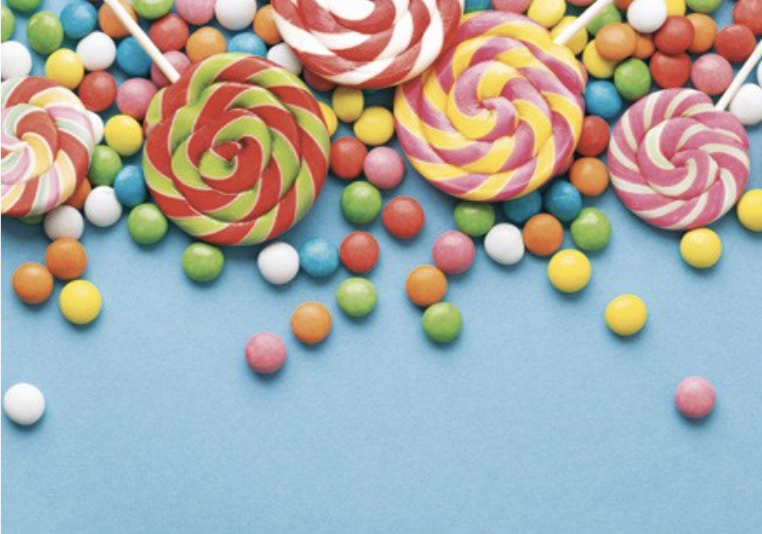
\includegraphics[width=0.9\textwidth]{bonbons.png}
\end{minipage}%

\vspace{10pt}

\noindent\hrulefill
\vspace{0.5cm}

\begin{center}
\textbf{Fin de l'interrogation — reliser avant de rendre.}
\end{center}

\end{document}
